% Autor: Benjamin Ternes
%
% FernUniversität in Hagen
% Lehrstuhl für Betriebswirtschaftsehre,
% insb. Entwicklung von Informationssystemen
% Leitung: Univ.-Prof. Dr. rer. pol. habil. Strecker
%
% Änderung nach >> GNU Public license <<
% 
% bibTeX abrufbar unter bibSonomy.org -- benji.ternes@gmail.com

\documentclass[12pt,a4paper,bibliography=totocnumbered,listof=totocnumbered,fleqn]{scrartcl}
\usepackage[ngerman]{babel}
\usepackage[utf8]{inputenc}
\usepackage[babel,german=guillemets,style=german]{csquotes}
\usepackage{amsmath}
\usepackage{amsfonts}
\usepackage{amssymb}
\usepackage{graphicx}
\usepackage{fancyhdr}
\usepackage{tabularx}
\usepackage{geometry}
\usepackage{setspace}
\usepackage[right]{eurosym}
\usepackage{acronym}
\usepackage{subfig}
\usepackage{floatflt}
\usepackage[usenames,dvipsnames]{color}
\usepackage{colortbl}
\usepackage{paralist}
\usepackage{array}
\usepackage{titlesec}
\usepackage{parskip}
\usepackage[right]{eurosym}
\usepackage[subfigure,titles]{tocloft}
\usepackage{pdfpages} 
\usepackage[pdfpagelabels=true]{hyperref}
\usepackage[round,authoryear]{natbib}

\makeatletter
\def\l@lstlisting#1#2{\@dottedtocline{1}{0em}{1em}{\hspace{1,5em} Lst. #1}{#2}}
\makeatother

\geometry{a4paper, top=27mm, left=30mm, right=20mm, bottom=35mm, headsep=10mm, footskip=12mm}

\hypersetup{unicode=false, pdftoolbar=true, pdfmenubar=true, pdffitwindow=false, pdfstartview={FitH},
	pdftitle={Beschichtungsverfahren},
	pdfauthor={Benjamin Ternes},
	pdfsubject={Studienarbeit},
	pdfcreator={\LaTeX\ with package \flqq hyperref\frqq},
	pdfproducer={pdfTeX \the\pdftexversion.\pdftexrevision},
	pdfkeywords={Beschichtungsverfahren,Benjamin Ternes},
	pdfnewwindow=true,
	colorlinks=true,linkcolor=blue,citecolor=black,filecolor=magenta,urlcolor=magenta
}
\pdfinfo{\today}

% -- Makro Programmierung -- Benjamin Ternes
\newenvironment{myquote}{\begin{quote} \small}{\end{quote}}
% -- 
\setlength{\skip\footins}{3em}

%\renewcommand{\labelitemi}{$-$}

\begin{document}

\titlespacing{\section}{0pt}{12pt plus 4pt minus 2pt}{-6pt plus 2pt minus 2pt}

% Kopf- und Fusszeile
\renewcommand{\sectionmark}[1]{\markright{#1}}
\renewcommand{\leftmark}{\rightmark}
\pagestyle{fancy}
\lhead{}
\chead{}
\rhead{\thesection\space\contentsname}
\cfoot{}
\lfoot{}
\rfoot{\ \linebreak Seite \thepage}
\renewcommand{\headrulewidth}{0.4pt}
%\renewcommand{\footrulewidth}{0.4pt}

% Vorspann
\renewcommand{\thesection}{\Roman{section}}
\renewcommand{\theHsection}{\Roman{section}}
\pagenumbering{Roman}


% ----------------------------------------------------------------------------------------------------------
% Titelseite
% ----------------------------------------------------------------------------------------------------------
\thispagestyle{empty}
\begin{center}
	%\includegraphics[scale=1]{Bilder/hs_os.png}\\
	\vspace*{2cm}
	\Large
	\textbf{Fachbereich}\\
	\textbf{Elektro- und Informationstechnik}\\
	FH Düsseldorf\\
	\vspace*{2cm}
	\Huge
	\textbf{Studienarbeit}\\
	\vspace*{0.5cm}
	\large
	über das Thema\\
	\vspace*{1cm}
	\Huge
	\textbf{Beschichtungsverfahren}\\
	\vspace*{2cm}
	
	\vfill
	\normalsize
	\newcolumntype{x}[1]{>{\raggedleft\arraybackslash\hspace{0pt}}p{#1}}
	\begin{tabular}{x{6cm}p{7.5cm}}
		\rule{0mm}{5ex}\textbf{Autor:} & Benjamin Ternes\newline benjamin.ternes@fernuni-hagen.de \\ 
		\rule{0mm}{5ex}\textbf{Prüfer:} & Prof. Dr. Prochotta \\ 
		\rule{0mm}{5ex}\textbf{Abgabedatum:} & 30.11.2013 \\ 
	\end{tabular} 
\end{center}
\pagebreak

% ----------------------------------------------------------------------------------------------------------
% Abstract
% ----------------------------------------------------------------------------------------------------------
\setcounter{page}{1}
\onehalfspacing
\titlespacing{\section}{0pt}{12pt plus 4pt minus 2pt}{2pt plus 2pt minus 2pt}
\rhead{KURZFASSUNG}
\section{Kurzfassung}

Verschleiß ereignet sich grundsätzlich überall dort, wo in Berührung befindliche Flächen durch Reibungseinfluss oder gegeneinander wirkend bewegt werden und wo korrosive Medien auf ungeschützte Flächen einwirken.
Standzeit und Beanspruchungsfähigkeit von Werkzeugen und verschiedenen Bauteilen sind somit wesentlich vom Verschleißverhalten dieser Materialien unter den Einsatzbedingungen bestimmt.
Die Reduzierung des Verschleißes, insbesondere von metallischen Werkstoffen, ist von großer wirtschaftlicher Bedeutung.
Hierzu eignen sich spezielle Schutzschichten, welche auf die Oberfläche aufgebracht werden und damit die Beschafffenheit der Werkstoffe verbessern bzw.\ entgegenwirken.
Damit wird die Widerstandsfähigkeit im wesentlichen erhöht, insbesondere auch die Gebrauchsdauer, oftmals auch in einer sonst erreichbaren Leistungssteigerung im Betrieb, besonders bei Werkzeugen.
In dieser Studienarbeit werden mit einer Einführung in den Problemkreis verschiedene Varianten der chemischen und physikalischen Schichtherstellung im Hinblick auf die Aufbringung von Verschleißschutztechniken auf Werkstoffe vorgestellt. Außer die klassischen Methoden des thermischen Spritzens werden auch neuere Methoden der ionen- und plasmagestützten Niedertemperaturverfahren ausführlich beschrieben.

\pagebreak

% ----------------------------------------------------------------------------------------------------------
% Verzeichnisse
% ----------------------------------------------------------------------------------------------------------
% TODO Typ vor Nummer
\renewcommand{\cfttabpresnum}{Tab. }
\renewcommand{\cftfigpresnum}{Abb. }
\settowidth{\cfttabnumwidth}{Abb. 10\quad}
\settowidth{\cftfignumwidth}{Abb. 10\quad}

\titlespacing{\section}{0pt}{12pt plus 4pt minus 2pt}{2pt plus 2pt minus 2pt}
\singlespacing
\rhead{INHALTSVERZEICHNIS}
\renewcommand{\contentsname}{II Inhaltsverzeichnis}
\phantomsection
\addcontentsline{toc}{section}{\texorpdfstring{II \hspace{0.35em}Inhaltsverzeichnis}{Inhaltsverzeichnis}}
\addtocounter{section}{1}
\tableofcontents
\pagebreak
\rhead{VERZEICHNISSE}
\listoffigures
\pagebreak
\listoftables
%\pagebreak
%\renewcommand{\lstlistlistingname}{Listing-Verzeichnis}
%{\labelsep2cm\lstlistoflistings}
\pagebreak

% ----------------------------------------------------------------------------------------------------------
% Abkürzungen
% ----------------------------------------------------------------------------------------------------------
\section{Abkürzungsverzeichnis}
\begin{acronym}[$Fe_{3}O_{3}(OH)_{2}$] 					% längste Abkürzung steht in eckigen Klammern
	\setlength{\itemsep}{-\parsep} 		% geringerer Zeilenabstand
	\acro{CVD}{Chemical vapor deposition (Chemische Gasphasenabscheidung)}
	\acro{PVD}{Physical vapor depositon (Physikalische Gasphasenabscheidung)}
\end{acronym}
\newpage


% ----------------------------------------------------------------------------------------------------------
% Inhalt
% ----------------------------------------------------------------------------------------------------------
% Abstände Überschrift
\titlespacing{\section}{0pt}{12pt plus 4pt minus 2pt}{-6pt plus 2pt minus 2pt}
\titlespacing{\subsection}{0pt}{12pt plus 4pt minus 2pt}{-6pt plus 2pt minus 2pt}
\titlespacing{\subsubsection}{0pt}{12pt plus 4pt minus 2pt}{-6pt plus 2pt minus 2pt}

% Kopfzeile
\renewcommand{\sectionmark}[1]{\markright{#1}}
\renewcommand{\subsectionmark}[1]{}
\renewcommand{\subsubsectionmark}[1]{}
\lhead{Kapitel \thesection}
\rhead{\rightmark}

\onehalfspacing
\renewcommand{\thesection}{\arabic{section}}
\renewcommand{\theHsection}{\arabic{section}}
\setcounter{section}{0}
\pagenumbering{arabic}
\setcounter{page}{1}

% ----------------------------------------------------------------------------------------------------------
% Einleitung
% ----------------------------------------------------------------------------------------------------------

% ----------------------------------------------------------------------------------------------------------
% Kapitel
% ----------------------------------------------------------------------------------------------------------
\section{Verschleiß}
\label{cha:verkor}

Verschleiß und Korrosion stellen die häufigste Ursache für die Oberflächenschädigung dar.
Der Materialabtrag ist entweder chemisch (Korrosion) oder mechanischer (Verschleiß) Natur und führt zu einer Zerstörung der Funktionstüchtigkeit eines Bauteils bzw.\ Werkstoffes durch Beeinträchtigung von Maßhaltigkeit und Festigkeit. Als Verschleiß definiert \texttt{DIN 50320}\footnote{~siehe~\ref{app:din50320}}

\begin{quote}
[\ldots] den fortschreitenden Materialverlust aus der Oberfläche eines festen Körpers, hervorgerufen durch mechanische Ursachen, d.h.\ Kontakt und Relativbewegung eines festen, flüssigen oder gasförmigen Gegenkörpers. [\ldots] (siehe~\ref{app:din50320})
\end{quote}

Hieraus folgt unmittelbar, dass bei Festkörperkontakt der Verschleißwiderstand grundsätzlich \emph{keine} Werkstoffeigenschaft, sondern eine Bauteilpaarungseigenschaft unter den jeweiligen Umgebungs- und Schmierungsbedingungen der Reibpartner darstellt, die in Fachkreisen als Systemeigenschaft bezeichnet wird.

\subsection{Verschleißarten und Verschleißmechanismen}
\label{sec:verver}

Die Anwendung des Systembegriffes auf \emph{tribologisch}\footnote{\textbf{Tribologie:} \emph{griechisch: Reibungslehre} befasst sich mit der wissenschaftlichen Beschreibung von Reibung, Verschleiß und Schmierung sowie der Optimierung von Reibungsvorgängen, die wie o.g. als wechselwirkende Oberflächen in relativer Bewegung oder als tribologisches System aufgefasst werden (siehe~\ref{fig:tribo_system}). Eine bekannte Rechengröße der Tribologie ist der Reibungskoeffizient $\mu$.} beanspruchte Bauteilpaarungen und deren Struktur hat die wissenschaftliche Systematik von Verschleißprozessen und die Entwicklung von Verschleißschutzmaßnahmen entscheiden beeinflusst \citep{bach2005moderne}. Bei der Reibung von Festen Körper findet in erster Linie eine mechanische Beanspruchung oberflächennaher Bereiche statt. Zudem spielt aber auch der Aufbau des Werkstoffinneren und das umgebende Medium eine wichtige Rolle. Unter Reibungsbedingungen ablaufende Oxidationsvorgänge können im Einzelfall wichtiger sein, als der mechanische Verschleiß. Hierbei wird eine direkte Beziehung zwischen Werkstoffhärt und Verschleißrate verhindert. Durch das Zusammenstoßen von Oberflächenunebenheiten verursacht durch die kurzzeitig großen Energiekonzentrationen den Ablauf besonderer tribochemischer und tribophysikalischer Prozesse in oberflächennahen Bereichen \citep{bach2005moderne}. Diese führen zur Bildung von Reaktions- oder Deckschichten bei der Reibung metallischer Werkstoffe, die für Art und Ausmaß der bei der Festkörperreibung stattfindenden Zerstörungsprozesse maßgebend sind. Die auf einer Oberfläche wirkenden Drücke sind abhängig von dessen Rauheitsprofil und können um mehrere Zehnerpotenzen über den nominellen Druck liegen. Bekanntlich haben ganz allgemein Werkstücke immer eine endliche Rauhtiefe. Gleiten solche Oberflächen aneinander, z.B.\ als Bauteile einer Maschine, so werden die Rauhigkeits-Spitzen der härteren Fläche die andere Fläche zerpflügen (Furchungsverschleiß, \emph{Abrasion}), Spitzen werden auch abgebrochen bzw.\ verformt. Die Berührungsflächen verschweißen (\emph{Adhäsion}) und legieren (Diffusion) an den Gleitflächen und werden danach wieder auseinander gerissen. Mit Hilfe der Makroskopie ist es möglich eine Reibung zu überwinden. Die Reibung, z.B.\ Lagerreibung bei Gleitlagern, wird vermindert durch einen Zwischenstoff wie Fette, Öle, Emulsionen, die auch zusätzlich als Kühlmittel wirken. Außerdem ist es möglich durch eine geeignete Trockenschmiersubstanz die Reibung zu reduzieren, dabei sind solche z.B.\ weiche Metalle wie $Au$, $Ag$, $Ir$, $Pb$, $Sn$ usw.\ , Verbindungen mit Schichtgitterstrukturen wie $MoS_{2}$, Graphit, usw.\ oder Kunststoffe wie Polyimide.\footnote{~siehe~Karl, Heinz. \textit{Tribologisches Verhalten keramischer Werkstoffe: Grundlagen und Anwendungen}. Ehningen bei Böblingen, 1993.} Verschleiß ist auch bei der Herstellung von Werkzeugen in der Materialbearbeitung eine sehr unerwünschte Begleiterscheinung. Die Auswirkungen der Reibung sind vielseitig, so zersetzen sich durch die entstehende Temperaturerhöhung viele konventionelle Schmierstoffe, verlieren somit ihre Schmierfähigkeit und erhöhen den Werkzeugverschleiß. 

\begin{figure}[h]
\centering
\includegraphics[scale=0.6]{img/tribo_system}
\caption{a) Orginalsystem, b) Ersatzsystem und c) Elementare Systemstruktur}
\label{fig:tribo_system}
\end{figure}

\subsubsection{Verschleißarten}
\label{sec:verart}

Einer Optimierung des Verschleißverhaltens geht die Analytische Betrachtung des tribologischen Systems (Tribosystem) voraus, d.h.\ die Untersuchung der Verschleißarbeit und der Verschleißmechanismen. Zu den Verschleißartern zählt \emph{Gleit-, Wälz-, Schwingungs-, Furchungs-, Spül- und Schrägstrahl-Verschleiß} sowie auch die \emph{Kavitationserosion}. Letztere stellt eine spezielle Verschleißart dar, die auf der Sogseite angeströmter Flächen auftritt. Der hier entstehende Unterdruck unterschreitet den Dampfdruck des strömenden Fluids und es kommt zur örtlichen Bildung von Blasen, die bei Druckerhöhung implodieren. In die dabei entstehenden Hohlräume stürzt nachströmende Flüssigkeit und trifft mit hoher Geschwindigkeit auf das Werkstück auf. Dieser Vorgang wiederholt sich mit hoher Frequenz. Die örtliche Zug-Druck-Wechsel-Spannung führt anfänglich zu einem mikroskopischen Schwingungsbruch, der sich zunehmend aufweitet und dann die Werkstoffoberfläche auflöst.  

\subsubsection{Verschleißmechanismen}
\label{sec:vermech}

Der Ablauf von Verschleißvorgängen hängt von den wirksamen Verschleißmechanismen ab. Der Verschleißkoeffizient

\begin{align}
k=\frac{W_{v}}{F_{n}\cdot s}
\end{align}

ist der Quotient aus dem Verschleißvolumen $W_{v}$ und der Normalkraft $F_{n}$ multipliziert mit dem Verschleißweg $s$. Dieser Koeffizient ist nur für abrasive Vorgänge konstant. Die nachfolgende Abbildung repräsentiert das Verschleißverhalten von Hartstoff-Verschleißschutzschichten den progressiven Verlauf der Oberflächenzerüttung.
Die Gesellschaft für Tribologie hat hierzu eine Tabelle veröffentlicht siehe~\ref{app:gft}.\footnote{~siehe~\url{http://www.gft-ev.de/}}

\begin{figure}[h]
\centering
\includegraphics[width=0.6\textwidth]{img/Linearer_Beitrag.pdf}
\caption{Linearer Verschleißbeitrag als Funktion der Betriebszeit bzw.\ des Verschleißweges für die Hauptverschleißmechanismen.}
\label{fig:verschleissbeitrag}
\end{figure}

\pagebreak

\textbf{Abrasion:}\\
Abrasion tritt in tribologischen Kontakten auf, wenn der Gegenkörper beträchtlich härter und rauher als der Grundkörper ist oder wenn harte Partikel in einen tribologisch beanspruchten Werkstoff eingedrückt werden. Durch Relativbewegung des Beanspruchungspartners kann aus dem weichen Grundkörper durch verschiedene Materialabtrennprozesse abrasiver Verschleiß entstehen (siehe~Abbildung~\ref{fig:abrasionsprozesse}).

\textit{Mikropflügen:}\\
Eine starke, plastische Verformung des Werkstoffes durch den abrasiven Gegenkörper erzeugt eine Materialaufwerfung am Riefenrand, Materialabtrag tritt nich zwingend auf.

\textit{Mikrospanen:}\\
Harte Rauhigkeitsspitzen der Abrasivpartikel zerspanen die Oberfläche, dabei werden Mikrospäne gebildet.

\textit{Mikrobrechen:}\\
Die überkritische Belastung eines spröden Werkstoffes durch einen Abrasivpartikel führt zu Rissbildung und Rissausbreitung, bis hin zum Materialabtrag.

\textit{Mikroermüdung:}\\
Wiederholtes Mikropflügen führt zu lokaler Werkstoffermüdung, die Materialabtrag zur Folge hat.
Dieser Teilprozess ist genaugenommen der Oberflächenzerüttung zuzuordnen.

\begin{figure}[h]
\centering
\includegraphics[scale=0.6]{img/tribo_system_III}
\caption{Abrasionsprozesse nach \citep{bobzin2013oberflchentechnik}.}
\label{fig:abrasionsprozesse}
\end{figure}

\pagebreak

\textbf{Adhäsion:}\\
Als Adhäsion versteht man eine stoffliche Wechselwirkung von Tribopaarungen (Bauteilspaarungen die in tribologischer Beanspruchung stehen).
Durch den Kontakt zweier Festkörperoberflächen bei hoher Pressung entstehen atomare Bindungen.
Bei einer erneuten Trennung der Triboelemente durch die Relativbewegung der Tribopaare, kommt es zum Ablösen von Material aus einer Oberfläche, welches auf der anderen Oberfläche haftenbleibt.
Bei metallischen Kontaktpartnern wird Adhäsion auch als Kaltverschweißung bezeichnet.
Jede Oberfläche weist eine Rauheit auf.
Berühren sich zwei Oberflächen, so stehen nur die Rauheitsspitzen der beiden Körper in direktem Tribokontakt.

\textbf{Tribochemische Reaktion:}\\
Tribochemische Reaktionen bewirken eine stoffliche Veränderung der Oberfläche von Tribokörpern.
Im Gegensatz zur Adhäsion findet hierbei eine chemische Reaktion an der Oberfläche nicht mit dem Gegenkörper, sondern mit dem Umgebungsmedium und bzw.\ oder dem Zwischenstoff statt.
Der Unterschied zur Korrosion besteht darin, dass die tribochemischen Reaktionen nur in der Kontaktfläche bei gleichzeitiger Relativbewegung stattfinden.
Die Reaktionsprodukte beeinflussen aktiv den Verschleißverlauf.
Die erhöhte chemische Reaktionsbereitschaft der Oberflächen führt zu tribochemischen Reaktionen wie der Tribooxidation.
Durch die veränderte chemische Zusammensetzung der Oberfläche verändern sich auch ihre Eigenschaften im Hinblick auf Festigkeitseigenschaften und Reibwerte.

\pagebreak

\textbf{Oberflächenzerrütung:}\\
Neben den statischen Belastungen können in tribologischen Systemen mechanische Wechselbelastungen auftreten, dir durch periodische Schwingungen beschrieben werden können (siehe~Abbildung~\ref{fig:wechsel}).
Dynamische Belastungen können zu Werkstoffermüdung der Randzone führen, die eine Rissbildung mit anschließenden Risswachstum zur Folge hat.
Hierbei ist der Verschleiß mit einer geringen Eindringtiefe zu bezeichnen.

\begin{figure}[h]
\centering
\includegraphics[scale=0.6]{img/tribo_system_IIII}
\caption{Zeitlicher Verlauf von mechanischen Belastungsfällen nach \citep{bobzin2013oberflchentechnik}.}
\label{fig:wechsel}
\end{figure}

\pagebreak
% ----------------------------------------------------------------------------------------------------------
% Kapitel
% ----------------------------------------------------------------------------------------------------------
\section{Korrosion}
\label{cha:korkor}

Unter dem Begriff \enquote{Korrosion} definiert \texttt{DIN EN ISO 8044}\footnote{~siehe~Anhang~\ref{app:korro}} 

\begin{myquote}
[\ldots] jede Reaktion eines Werkstoffes mit seiner Umgebung, die eine messbare Veränderung seines Zustandes bewirkt und zu einer Beeinträchtigung der Funktion eines aus diesem Werkstoff gefertigten Bauteils führt [\ldots]
\end{myquote}

Ein metallischer Werkstoff korrodiert, wenn er sich von seiner Oberfläche ausgehend durch unerwünschte chemische bzw.\ elektro-chemische Angriffsmittel verändert. Dieses korrosiven Medien können gasförmig, flüssig oder auch fest sein. Der ausgehende metallische Zustand des Elements geht unter der Einwirkung verloren und es entstehen unerwünschte Korrosionsprodukte. Bekanntlich korrodieren Eisen und gewöhnlicher Stahl bereits an feuchter Luft. Dabei wird Eisen aus seinem metallischen Zustand \emph{vollständig} in die nicht metallische Verbindung Ferrohydroxid $Fe(OH)_{2}$ übergeführt und durch Sauerstoff Aufnahme entsteht dann das rostbraune Korrosionsprodukt Eisen(II,III)-Oxidhydrat $Fe_{3}O_{3}(OH)_{2}$, das allgemein als \enquote{Rost} bezeichnet wird. \emph{Atmosphärische Korrosion} tritt bei sog.\ unedlen Nichteisenmetallen unter dem Einfluss von Sauerstoff, Wasserdampf, Kohlendioxid und anderen Gasen auf. In vielen Fällen beschränkt sich die Korrosion dabei auf die Oberfläche, an der sich eine Schutzschicht bildet, die, sofern nicht mechanisch abgebaut wird, das unterliegende Metall vor weiterem Angriff bewahrt (z.B.\ $Al/Al_{2}O_{3}$ bzw.\ $Zn/3Zn(OH)_{2}$). In sehr feuchten Gebieten, Tropenluft, in salzhaltiger Seeluft oder in der Industrieluft mit höheren $CO_{2}$-,~$SO_{2}$- und $H_{2}S$-Gehalten tritt bei den meisten metallischen Werkstoffen eine verstärkte Korrosion auf. Korrosion in flüssigen Medien ist vor allem in Säuren, Basen und Salzlösungen zu finden. Am weitesten verbreitet und bekannt ist die Korrosion durch Meerwasser. Prinzipiell ist Korrosion abhängig von der korrosiven Umgebung, dem Korrosivmedium, dabei wird zwischen Heißgaskorrosion und elektrolytischer Korrosion unterschieden. Außerdem werden Korrosionsformen nach der Art des Angriffs als flächenhaft, selektiv, unter Reaktion einzelner Gefüge-, Schichtbestandteile oder unter Ausbilden von Rissen unterschieden.

Die eigentliche Ursache jeder Korrosion ist das Bestreben des Werkstoffes unter den gegebenen Verhältnissen in einen stabilen Energiezustand mit möglichst niedrigem Potential überzugehen.
Die meisten Metalle werden aus natürlichen vorkommenden Verbindungen, den Erzen (Metalloxide, Metallhydroxide, Metallkarbonate, Metallsulfide usw.\ ), unter erheblicher Energiezufuhr gewonnen.
So werden für die Herstellung von Stahl $29.4$Mio.\ $kJ/t$ Energie benötigt.
Das so gewonnene Metall befindet sich in einem unnatürlichen, thermodynamischen Zwangszustand hohen Potentials.
Das Bestreben der Metalle ist es, aus dem energiereichen, metallischen Zustand in den energieärmeren, nicht metallischen Zustand, zurückzukehren.

\textbf{Beispiel:}\\
Im Hochofenprozess wird Eisen unter hohem Energieaufwand durch Reduktion seiner oxidischen Erze, wie z.B.\ $Fe_{2}O_{3}$ (Roteisenerz) oder $Fe_{3}O_{4}$ (Magneteisenstein) gewonnen (Verhüttung):

\begin{align*}
Fe_{2}O_{3} + 3CO + 23.9kJ \rightarrow 2Fe + 3CO_{2}\\
Fe_{3}O_{4} + 4CO + 18.1kJ \rightarrow 3Fe + 4CO_{2}
\end{align*}

Durch Reaktion mit der Umgebung (Verrostung) versucht das so erzeugte Eisen seinen thermodynamischen Zwangszustand wieder zu verlassen und sich in Rost zu verwandeln, der chemisch gesehen dem Eisenerz identisch ist.
Die Neigung der Metalle mit dem Umgebungsmedium zu reagieren, ist bei unedleren Metallen eher der Fall, als bei edlen Metallen wie Gold, Silber, Platin.

\subsection{Zusammenfassung}

Neben der Korrosion stellt der Verschleiß die häufigste Ursache für eine Oberflächenschädigung dar. Dabei ist der Materialabtrag immer auf eine mechanische Beanspruchung der Oberfläche zurückzuführen. Durch den Materialabtrag der Oberfläche wird das Bauteil in seiner Funktionstüchtigkeit, Festigkeit und Maßhaltigkeit beeinträchtigt. Oberflächenschutzschichten bieten durch die Trennung der Bauteilfunktionen die Möglichkeit, Teilbereiche entsprechend der jeweiligen Belastung gezielt zu schützen. Der Auswahl des Beschichtungsverfahrens muss einer ausführlichen Analyse unterzogen werden, so dass vorliegende Probleme spezifiziert werden können.

Im Unterschied zum Verschleiß ist für die Korrosion nicht zwangsläufig eine Belastung des entsprechenden Bauteils erforderlich, kann also auch an Ersatzteilen in einem Lager zu Bauteilbeschädigungen führen. Korrosionsvorgänge an beschichteten Bauteilen können unter Einsatzbedingungen über Bauteilschädigungen bis hin zu deren Versagen führen \citep{bach2005moderne}. Je nach vorliegenden Korrosionsmechanismus kann die Schädigung als Korrosion auf der Beschichtung oder auch darunter ablaufen. Es kann Schichtablösung stattfinden oder auch eine von außen unsichtbare Korrosion des Grundwerkstoffes erfolgen, die unter Belastung möglicherweise zum Bruch des Bauteils führt.

\pagebreak
% ----------------------------------------------------------------------------------------------------------
% Kapitel
% ----------------------------------------------------------------------------------------------------------
\section{Thermisches Spritzen}
\label{sec:thermspritzen}

\subsection{Thermische Spritzverfahren}

Thermische Beschichtungsverfahren sind Techniken zum Beschichten von Bauteilen mit Materialien unterschiedlicher Art zum Schutz gegen Verschleiß, Korrosion, zum Erzielen von elektrischen oder magnetischen Eigenschaften und vieles mehr. Der Spritzzusatz in Pulver, Draht- oder Stabform, wird einer energiereichen Wärmequelle zugeführt und darin an- oder aufgeschmolzen. Durch einen Gasstrom werden die Partikel auf das gewünschte Bauteil aufgeschleudert. Das Substrat unterliegt während des Beschichtungsprozesses i.d.R.\ nur einer geringen thermischen Belastung \citep{bach2005moderne}.

\begin{figure}[h]
\centering
\includegraphics[scale=0.7]{img/prinzip_des_thermischen_Spritzens}
\caption{Prinzip des thermischen Spritzens.}
\label{fig:thermischspritzen}
\end{figure}

Die Verfahren des thermischen Spritzens werden in Abhängigkeit von der Wärmeeinbringung unterschieden.
Die am weitesten verbreiteten Verfahren sind das Flammspritzen, das Hochgeschwindigkeitsflammspritzen, das Lichtbogenspritzen und das Plasmaspritzen.
Wesentliche Vorteile der thermischen Spritzverfahren sind \citep{bach2005moderne}:

\begin{itemize}
	\item es sind Schichten aus nahezu allen Werkstoffen herstellbar
	\item geringe thermische Belastung des Werkstückes
	\item lokale sowie verstärkte Beschichtung möglich
	\item Verfahren sind mobil anwendbar
	\item es können nahezu alle Werkstoffe beschichtet werden
	\item hohe Auftragsraten (Schichtdicke: 20$\mu m$ --- mehrere $mm$)
\end{itemize}

\textbf{Übersicht über die Unterteilung der Verfahren des thermischen Spritzens:}\\

\begin{figure}[h]
\centering
\includegraphics[scale=0.7]{img/verfahren_des_thermischen_spritzens}
\caption{Verfahren des thermischen Spritzens.}
\label{fig:thermischspritzenverfahren}
\end{figure}

\subsubsection{Entstehung einer thermisch gespritzten Schicht}

Die Eigenschaften einer Spritzschicht werden maßgeblich von den Spritzbedingungen und vom verwendeten Spritzzusatzwerkstoff beeinflusst.
Der Schichtaufbau und die Schichtaufbau und die Schichtstruktur der gespritzten Schicht bestimmen den Charakter und die Eigenschaft des Systems Schicht --- Substrat.
Allen thermischen Spritzverfahren haben gemeinsam, dass hocherhitzte Werkstoffpartikel einen Weg von der Spritzpistole zur Substratoberfläche zurücklege, auf dem sie der umgebenden Atmosphäre ausgesetzt sind und unter Umständen mit den hierin enthaltenen Gasen reagieren.

Aufgrund der konzentrierten Wärmeeinbringung in das Partikel und der Flugphase durch die umgebende Atmosphäre kann es durch folgenden Reaktionen zu einer Veränderung der Zusammensetzung und der Struktur der gespritzten Schicht kommen:\\

\begin{itemize}
	\item selektives Verdampfen einer Komponente
	\item Reaktionen von Metallverbindungen
	\item Bildung nicht flüchtiger Metallverbindungen wie Oxide, Nitride und Hybride in Anwesenheit von $O_{2}$, $N_{2}$, $H_{2}$ (insb.\ bei reaktiven Metallen)
\end{itemize}

Von besonderer Bedeutung ist die oberflächliche Oxidation metallischer Spritzpartikel auf ihrem Weg zum Substrat.
Die sich bildenden Oxide sind mitverantwortlich für die Lamellenbildung der Spritzschicht.
Hierdurch kann es z.T.\ zu einem Anwachsen der Schichthärte sowie der Verschleißbeständigkeit der Schicht kommen.
Durch Verlegen des Spritzprozesses in eine Inertgasatmosphäre, z.B.\ Stickstoff oder Argon, lässt sich insb.\ das Bilden von Metalloxiden verhindern.
So weisen in einer Inertgasatmosphäre hergestellte Spritzschichten im allgemeinen ein homogeneres Gefüge mit gleicher chemischer Elementzusammensetzung wie der zugeführte Spritzzusatzwerkstoff auf.

Als Substratvorbereitung dient meist ein Strahlvorgang, der die zu beschichtende Oberfläche aktiviert, dekontaminiert und effektiv aufrauht.
Die Spritzschicht baut sich durch den Aufprall der Partikel auf, die sich auf der Substratoberfläche verformen bzw.\ ausbreiten und durch Wärmeabgabe an das Werkstück erstarren.
Thermisch gespritzte Schichten weisen eine lamellare Schichtstruktur auf und sind je nach eingesetzten Spritzverfahren und -werkstoff mehr oder weniger porös, mikrorissig, heterogen und anisotop.
Außerdem enthalten diese Schichten nicht vollkommen aufgeschmolzene oder vor dem Auftreffen auf die Substratoberfläche wieder erkaltete sowie mit Umgebungsgasen reagierte Partikel.

Die Schicht haftet durch mechanische Verklammerung sowie lokal durch van der Waals- oder chemische Bindungen und durch chemisch-metallchirugische Wechselwirkungen an der Substratoberfläche.

\subsection{Nachbehandeln von thermisch gespritzen Schichten}

Durch thermisches Spritzen (siehe~Kapitel~\ref{sec:thermspritzen}) aufgetragene Schichten zeichnen sich herstellungsbedingt durch charakteristische, oft unerwünschte Merkmale aus, die ihr \emph{Einsatzgebiet} einschränken. Unter den Merkmalen können sein:

\begin{itemize}
	\item hohe Porosität
	\item Unebenheit
	\item Ungleichmäßigkeit der Struktur und der chemischen Zusammensetzung
	\item Eigenspannung
	\item geringe Haftung mit dem Grundwerkstoff
\end{itemize}

Um die gewünschten Schichteigenschaften zu optimieren, wird eine sog.\ \emph{Nachbehandlung} angewandt, welche sowohl auf die geforderten Schichteigenschaften, als auch auf die Werkstoffe von Schicht und Substrat abgestimmt sein muss. Es gibt unterschiedliche Verfahren um eine Nachbehandlung durchzuführen:

\begin{itemize}
	\item mechanische
	\item thermische
	\item thermo-mechanische
	\item Strahlverfahren
\end{itemize}

Aufgrund des Umfanges wird das Strahlenverfahren im weiteren der Ausarbeitung nicht bearbeitet. Das Strahlenverfahren ist ein sehr effizientes Verfahren zur Nachbehandlung.

\subsubsection{Mechanische Verfahren}

Spanen thermisch gespritzter Schichten, wie z.B.\ das Drehen und das Schleifen, ist für die Herstellung von Gleitflächen mit verschleißbeständigen Schichten notwendig. Das Erzielen eines bestimmten Endmaßes und einer bestimmten Oberflächenqualität erfordert ein Nachbearbeiten, das sowohl vom Werkstoff als auch vom Beschichtungsverfahren abhängig ist. Ungeeignete Parameter bei der Oberflächenqualität sowie beim Beschichtungsverfahren führen zu einer Zerstörung des Schichtsystems und zum Versagen des Werkstückes. Gründe dafür sind eine begrenzte Haftung der Schichten durch fremdartige Einschlüsse wie z.B.\ Oxide, Karbide oder Nitride, welche abhängig vom Spritzverfahren zu einem gewissen Grad in der Schicht vorhanden sind. Die mechanische Nachbehandlung erlaubt es, neben der Oberflächenbearbeitung der Schicht auch ihre Volumeneigenschaften zu beeinflussen. Insbesondere ist es möglich, bei hoch Porösen Schichten die Porösität der Schicht durch eine mechanische Nachbehandlung zu verringern. Diese Nachbehandlung ist vor allem bei Korrosionsschutzschichten von Bedeutung, weil eine Schutzwirkung nur bei vollständiger Dichtheit zu erzielen ist. 

Das Verdichten von Überzügen erfolgt mit unterschiedlichen Verfahren, die sich durch das Aufbringen von Druckkräften auszeichnen. Eines der Verfahren ist das \emph{Überrollen} der aufgetragenen Schicht mit speziellen Wälzkörpern unter einer definierten Andruckkraft.\footnote{Juchmann, P.:\ \textit{Beitrag zur technologischen Eigenschaftserweiterung von Magnesium-Werkstoffen durch Lithium}, Dissertation, Universität Hannover, 1999.} Die plastische Verformung in dem Bereich unter dem Wälzkörper bewirkt dabei das Verdichten einer Beschichtung. Es resultiert eine Überlappung einzelner Spuren des beschichteten Bereiches.

Ein anderes Verfahren der mechanischen Nachbehandlung ist das \emph{Kugelstrahlen}. Als Strahlmittel dienen bei diesem Verfahren kugelförmige Partikel aus Glas, Keramik oder Stahl mit einem Durchmesser im Bereich etwa $0.1$ bis $3mm$ \citep{bach2005moderne}. Die mit dem Gasstrom beschleunigten Partikel erreichen je nach Anwendung eine Geschwindigkeit von bis zu $200\frac{m}{s}$. Die hohe kinetische Energie der beschleunigten Partikel erlaubt es, die Schichtporosität sowie die Oberflächenrauheit deutlich zu reduzieren. Die Wahl des Strahlenmittelwerkstoffs richtet sich nach dem jeweiligen Verwendungszweck unter Berücksichtigung der Härte und Zersplitterungsneigung der Kugeln. Bei ausreichender Zähigkeit muss die Härte des Strahlmittels deutlich über der des zu behandelnden Schichtmaterials liegen, um unerwünschte Verformungen der Kugeln zu vermeiden.

Ein weiteres Verfahren zur Verbesserung der Schichtqualität besteht aus dem \emph{simultanen Ablauf von Beschichtungs- und Strahlprozess}. Dabei bewegt sich die Kugelstrahlkanone relativ zum Werkstück hinter der Beschichtungskanone, so dass die auf die Oberfläche aufprallenden Beschichtungspartikel sofort nach dem Erstarren mit den Kugeln gestrahlt und verdichtet werden \citep{hofmann2010verfahren}. Dieses Verfahren stellt sicher, dass nicht nur der oberflächennahe Bereich, sondern auch der gesamte Schichtbereich komprimiert wird. Die resultierenden Schichten weisen einen geringeren Porenanteil und eine deutlich reduzierte Eigenspannung auf.    

\subsection{Anwendungen}

\textbf{Korrosionsschutz:}
\begin{itemize}
	\item Erstellung passiver Korrosionschutzschichten mit chemisch beständigen Werkstoffen (z.B.\ Korrosionsschutz in der chemischen Industrie durch Kunststoffe)
	\item Erstellung von Gleitschichten: Verringerung der Oberflächenrauhigkeit zur Verminderung der Reibung oder Applikation von selbstschmierenden Schichten (z.B.\ Einsatz mikroporöser Schichten mit eingelagerten Schmiermittel)
\end{itemize} 

\textbf{Instandsetzung:}
\begin{itemize}
	\item Neuaufbau verschlissener Oberflächen (z.B.\ Reparatur von Turbinenschaufeln durch Beschichtung mit legierten Stählen)
\end{itemize}

\textbf{Elektrische Kontaktierung/Isolation:}
\begin{itemize}
	\item Beschichtung mit elektrisch leitfähigen bzw.\ isolierenden Werkstoffen (z.B.\ Isolationsschichten aus oxidkeramischen Werkstoffen)
\end{itemize}

\textbf{Luftfahrtindustrie:}
\begin{itemize}
	\item Brennkammerauskleidung
	\item Turbinenbeschichtung
\end{itemize}

\textbf{Allgemeiner Maschinenbau:}
\begin{itemize}
	\item Verschleißschutz (z.B.\ Wellenlagerflächen, Kalanderwalzen, Zinkbadrollen, Werkzeugbeschichtungen)
\end{itemize}

\textbf{Chemie- und Kraftstoffindustrie:}
\begin{itemize}
	\item Verschleiß- und Korrosionsschutz (Erdöl- und Erdgasfördereinrichtungen, Pipelines)
\end{itemize}

\textbf{Automobilindustrie:}
\begin{itemize}
	\item Verschleißschutz (Kolbenringe, Zylinderlaufflächen, Ventilflächen bei Dieselmotoren)
\end{itemize}

\pagebreak
% ----------------------------------------------------------------------------------------------------------
% Kapitel
% ----------------------------------------------------------------------------------------------------------
\section{Lichtbogenspritzen}

Das Lichtbogenspritzen wurde erstmalig im Jahre 1915 vom Schweizer \enquote{M. U. Schoop} beschrieben. Anfängliche Prozessinstabilitäten konnten mit der Entwicklung geeigneter Stromquellen beseitigt werden. Maßgeblich für die industrielle Einsetzbarkeit war das Erforschen der wissenschaftlichen Grundlage dieses thermischen Spritzverfahrens in den 50er und 60er Jahren. Trotz der Einführung neuer Hochenergieverfahren, wie Plasma-, Detonations- und Hochgeschwindigkeitsflammspritzen, hat sich das Lichtbogenspritzen aufgrund seiner Wirtschaftlichkeit durchgesetzt. Durch die Anlagenvielfalt und ein zunehmendes Angebot an geeigneten Zusatzwerkstoffen weist dieses ein breites Einsatzspektrum auf. 

\subsection{Verfahrensprinzip}

Beim Lichtbogenspritzen werden zwei metallische Drähte gleicher oder unterschiedlicher Art \emph{(Pseudo-Legierung)} mit geregelter Drahtvorschubgeschwindigkeit in die Spritzpistole bewegt. Die Stromübertragung erfolgt meist über kupferne, kontaktgebende Drahtführungen, die in einem Winkel von etwa 30$^\circ$ zueinander angeordnet sind. Nach dem aktivieren des Drahtvorschubes, laufen beide metallischen Drähte aufeinander zu, bis zur Berührung. An dieser Stelle liegt von allen Teilwiderständen im Stromkreis der geringste Ohm'sche Widerstand vor. Infolge des hohen kurzschlussstromes tritt eine starke Erwärmung auf, wodurch Metall verdampft und sich der Lichtbogen entzündet. Die Spannung in der Stromquelle fällt zunächst auf einen geringeren Wert ab, während der Strom auf den sog.\ Kurzschlussstrom ansteigt.

\pagebreak

\begin{figure}[h]
\centering
\includegraphics[scale=0.7]{img/libo.jpg}
\caption{Verfahrensprinzip beim Lichtbogenspritzen.}
\label{fig:libo}
\end{figure}

Die Temperaturen während des Lichtbogenspritzens erreichen etwa 4000$^\circ$. Der Werkstoff wird an-, ab- oder aufgeschmolzen und ein aus einer Düse austretender Gasstrom (i.d.R.\ Druckluft) zerstäubt das Schmelzgut, beschleunigt die Partikel und schleudert sie auf die zu beschichtende Oberfläche. Das Verfahren ist prinzipiell auch mit drei bzw.\ vier Drähten als Mehrdrahtlichtbogenspritzen anwendbar siehe \citep{bach2005moderne}.

\subsubsection{Werkstoffe und Anwendungen}

Als klassische Werkstoffe beim Lichtbogenspritzen stellen sich in Form von schmelz- oder pulvermetallurgisch hergestellten Massivdrähten Kohlenstoffstähle, Chrom- und hochlegierte Stähle, Lagerbronzen und Nichteisenmetalle \citep{bach2005moderne} und \citep{bobzin2013oberflchentechnik}.
Verfahrenstypische Anwendungen sind der Korrosionsschutz im Off-Shore-Bereich und im Stahlbau, die Herstellung von Verschleißschutzschichten sowie deren Reperatur nach Verschleißschäden und die Metallisierung von Kunststoffgehäusen.
Aber auch das Aufbringen von Haftgrundschichten (NiCr, NiAl) sowie die Beschichtung im Automobilbereich sind Anwendungsgebiete.
Durch hochentwickelte Anlagentechnik können bisher plasmagespritzte Metallschichten in vergleichbarer Qualität lichbogengespritzt werden.
Pseudo-Legierungen entstehen durchs gleichzeitige Verspritzen zweier oder mehrerer verschiedener Metalle, wie z.B.\ Stahl und Bronze für den Einsatz als hochbeanspruchte Lager.

\pagebreak

\begin{table}[h]
\centering
\begin{tabular}{p{3cm} p{11cm}}
\hline
\\
Werkstoffe		&	Anwendungen
\\
\hline
\\
Al,AlMg	&	Reperatur von Al-Teilen, Auspufftöpfe (Massenproduktion), Wärmetauscher, Off-Shore-Technik: Rohrleitungen und Ölbohrplattformen, Kessel, Brammenmarkierung, Fleischereimaschinen\\
Cu			&	Widerstände, Kondensatoren, Leiterbahnen auf Kunststoff- und Keramiksubstraten\\
Mo			&	Haftschicht auf Stahl, Verschleißschutzschichten\\
NiCr, NiAl	&	Abschirmung (Röntgenstrahlen), Haftschicht für Plasmaspritzschichten\\
NiCuMn		&	Schiebergehäuse, Armaturenteile, Pumpenwelle\\
Sn-Leg.		&	Gleitlager, Kondensatoren\\
Stahl		&	Verschleißschutz- und Reperaturschichten: Plunger, Getriebegehäuse, Aluminiumteile (Ventile)\\
Zn			&	Brücken und Stahlkonstruktionen, Kessel, Tore, Großrohre (Pipelines), Gießformen, Karosserinähte\\
\\
\hline
\end{tabular}
\caption{Werkstoffe und Anwendungsbeispiele für das Lichtbogenspritzen siehe hierzu \citep{bach2005moderne}.}
\end{table}

Als zu beschichtende Werkstoffe eignen sich alle technischen Metalle und Legierungen, die sich durch Druckluftstrahlen genügend aufrauhen lassen, d.h.\ deren Rockwell-Härte,\footnote{~Rockwell ist eine internationale Maßeinheit für die Härte technischer Werkstoffe. Kürzel: HR besteht aus \textbf{H}ardness \textbf{R}ockwell als Kennzeichnung des Verfahrens gefolgt einem weiteren Buchstaben der die Skala und damit die Prüfkräfte und Prüfkörper angibt (Welle im Getriebe hat die Härte 48HRC).} d.h.\ deren Rockwell-Härte kleiner als 55HRC ist.
Die mit diesem Verfahren erzeugten Spritzschichten sind gekennzeichnet durch eine lamelle Struktur, je nach Werkstoff ausgeprägte Haftung zum Substrat, starken Abbrand von Legierungsbestandteilen (insb.\ Kohlenstoff, Mangan, Chrom) sowie Porosität von 2\% - 10\% .
Das Versiegeln von lichtbogengespritzten Schichten durch organische bzw.\ anorganische Siegler erhöht den Korrosionsschutz und wird bei Aluminium sogar empfohlen.
Die Flüssigkeit dringt in die poröse Schicht ein und versiegelt diese nach dem Trocknen und Aushärten an der Luft oder im Ofen.

\subsubsection{Schichtstruktur}

Die Teilchenbildung und das kinetische Verhalten der Spritzpartikel auf ihrem Flugweg hängen vom Zersträubergas und des metallischen Spritzzusatzwerkstoffes ab, hauptsächlich doch von der verwendeten Spritzanlage, dem Düsensystem, dem Zersträuberdruck $P$, der Spannung $U$, der Stromstärke $I$ und dem Abstand zum Werkstück.
Eine wesentliche Verbesserung hinsichtlich des Zerstäubens der Schmelze brachte die Entwicklung geschlossener Zersträubersysteme.
Dabei kann die Spritzpistole von einem offenen Düsensystem in ein geschlossenes umgerüstet werden.

\begin{figure}[h]
\centering
\includegraphics[scale=0.6]{img/libo_spritzen}
\caption{Offenes (oben) und geschlossenes (unten) Düsensystem einer Lichtbogenspritzpistole, Fa. OSU, Typ LD/U2 (Querschnitte von oben; Vorderansicht).}
\end{figure}

Die beiden Düsensysteme unterscheiden sich in ihrer technischen Ausführung, beim geschlossenen System hat man eine zusätzliche Düsenscheibe die sich über der Drahtelektrode befindet.
Hohe elektrische Leistungen bei geringen Drahtvorschubgeschwindigkeiten und daraus resultierend hohe spezifische Energien ($q > 40kJ/kg$) führen infolge einer höheren Temperatur und der damit verbunden niedrigen Vikosität der Schmelze zum Ausbilden kleinerer Partikel sowie einem höheren Oxidgehalt der Schicht.
Beim Verarbeiten von Stahl kommt es darüber hinaus bei hohen elektrischen Strömen zum Abbrand von Legierungselementen (Cr, C, Mn).

\begin{figure}[h]
\centering
\includegraphics[scale=0.7]{img/libo_spritzen_II}
\caption{Lichtbogenspritzanlage im Betrieb.}
\end{figure}

Der Zersträuberdruck stellt eine der wesentlichen Einflussgrößen auf die Partikelgröße und die sich einstellende Schichtstruktur.
Mit zunehmenden Zersträuberdruck entstehen kleinere und schnellere Partikel, was zu einem homogenen Schichtaufbau führt \citep{bobzin2013oberflchentechnik}.

\begin{figure}[h]
\begin{minipage}[t]{6cm}
\includegraphics[width=0.9\textwidth]{img/libo_schicht2}
\end{minipage}
\hfill
\begin{minipage}[t]{6cm}
\includegraphics[width=0.9\textwidth]{img/libo_schicht3}
\end{minipage}
\caption{Links: Offenes Düsensystem, Querschliff einer lichtbogengespritzten Stahlschicht (1\% -C-Stahl), Fa. Miller/Praxair BP 400 (HV Düse).Rechts: Geschlossenes Düsensystem, Querschliff einer lichtbogengespritzten Zinkschicht, Fa. Sulzer Metco Smartac (HV Düse).}
\end{figure}

Jüngere Anlagentechnische Entwicklungen zum verbessern der Schichtstruktur zielen auf eine Maximierung der Gasgeschwindigkeit ab.
Durch das verwenden von Hochgeschwindigkeitsdüsen sind sehr dichte Lichtbogenspritzschichten herstellbar.
\pagebreak

\subsection{Vor- und Nachteile}

Ein Nachteil des Lichtbogenspritzens stellt die Beschränkung des Spritzzusatzes auf elektrisch leitende Drähte dar.
Darüber hinaus sind aufgrund der enstehenden Spritzstäube, der großen Lärmentwicklung (110dB) sowie der hohen ultravioletten und infraroten Strahlung spezielle Arbeitssicherheitsmaßnahmen erforderlich.
Die technischen Vorteile liegen in der hohen Auftragsrate, der Herstellungsmöglichkeit mehrerer Millimeter dicker Schichten, der einfachen Handhabung und der im Vergleich zu anderen Spritzverfahren geringeren Anlagekosten (sowohl Anschaffung als auch Betriebskosten).
Das Lichtbogenspritzen zählt zu den wirtschaftlichsten Verfahren hinsichtlich der Energieausnutzung zum Aufschmelzen des Werkstoffes in der thermischen Spritztechnik.

\pagebreak
% ----------------------------------------------------------------------------------------------------------
% Kapitel
% ----------------------------------------------------------------------------------------------------------
\section{Plasmaspritzen}

Der Einsatz des Plasmas als Energiequelle geht auf Entwicklungen aus den 1920er bis 1930er Jahren zurück und wurde um 1950 zur Industriereife gebracht.
Charakteristisch für das Plasmaspritzen sind hohe Plasmatemperaturen von bis zu $T_{p}=20000K$, die die Verarbeitung jedes kongruent schmelzende Werkstoffes erlauben.
Mit dem Plasmaspritzen konnten damit erstmals auch hochschmelzende keramische Werkstoffe verarbeitet werden.
Von 1960 bis in den späten 90er Jahren erfolgte eine enorme Wachstumsphase in der Thermischen Spritztechnologie.
Durch den immer größer werdenden Bedarf an keramischen Wärmedämmschichten aus Yttriumoxid stabilisierten Zirkonoxid für die Luft- und Raumfahrtindustrie konnte sich das Plasmaspritzverfahren endgültig durchsetzen (Prozesstemperaturen: $T=12000-15000K$).
Plasmaspritzverfahren werden i.d.R.\ unter Atmosphärischen Bedingungen ausgeführt.

\textbf{Andere Verfahrentypen:}
\begin{itemize}
	\item Atmosphärisches Plasmaspritzen (APS)
	\item Vakuumplasmaspritzen (VPS)
	\item Niederdruck (LPPS)
	\item Schutzgasmantel (SPS)
\end{itemize}

Der Begriff \enquote{Plasma} wurde 1923 von dem amerikanischen Physiker und Chemiker \enquote{Irving Langmuir} eingeführt.

\begin{myquote}
Unter Plasma versteht man ein ionisiertes, heißes Gas aus Ionen, Elektronen und neutralen Teilchen, die sich durch die ständige Wechselwirkung untereinander und mit Photonen in verschiedenen Energie- und Anregungszuständen befinden. Plasmen besitzen damit eine hohe elektrische Leitfähigkeit. Ein Plasma ist nach außen quasineutral, d.h.\ es hat im Mittel die gleiche Anzahl von positiven und negativen Ladungen. (frei zitiert nach Prof.~Dr.~U.~Hahn, FH~Dortmund. Vorlesung: Werkstoffe der Elektrotechnik.)
\end{myquote}
\pagebreak

\subsection{Verfahrensprinzip}

\begin{figure}[h]
\centering
\includegraphics[scale=0.3]{img/plasma_I}
\caption{Schematischer Aufbau eines Einkathoden-Plasmagenerators nach \citep{bobzin2013oberflchentechnik}.}
\label{fig:plasmaprinzip}
\end{figure}

An der Düsenmündung rekombiniert das Gas, sobald eine weitere Energiezufuhr nach Passieren des Lichtbogens entfällt.
Dabei werden große Energiemengen freigesetzt, die eine explosionsartige Expansion des Gases durch die Düse zur Folge haben.
Die elektrische Energie des Lichtbogens wird somit in thermische und kinetische Energie des Plasmastrahls umgewandelt, die zum Aufschmelzen und Beschleunigen der Spritzpartikel verwendet werden siehe \citep{thermal2008}.

Mittels geeigneter Kühlmaßnahmen kann die Substrattemperatur in einem Bereich von $T_{s}=70-200^\circ C$ gehalten werden.
Prozessparameter liegen bei Stromstärken von $I=400-600A$, einer Bruttoleistung von $P=20-200kW$, einer Kühlleistung von $P_{K}=15-25kW$ und einen Volumenstrom des Plasmagasgemischs $\dot{V}=40-60$SLPM\footnote{~\textbf{SLPM:} Standard Liter pro Minute, die Einheit SLPM für den Gasmengenstrom $Q$, kurz slpm oder slm, ist ein Maß für die Molekülmenge, die pro Zeiteinheit und unter Normbedingungen durch einen Querschnitt fließt. Die Einheit ist folgendermaßen definiert: $1 slpm = \frac{1013.35 mbar \cdot 1l}{60s} = 16.8875 \frac{mbar\cdot l}{s}$. Im SI-Einheitensystem umgerechnet ergibt das: $1.68875 \frac{Pa\cdot m^{3}}{s}$.}
Als Plasmagase werden Argon, Helium, Stickstoff oder Wasserstoff bzw.\ Mischungen daraus eingesetzt.

Mit dem Verfahren des APS werden neben Metallen und Legierungen für mittlere Korrosions- und Verschleißbeanspruchungen insb.\ keramische Werkstoffe verarbeitet.
Die gängisten keramischen Werkstoffsysteme sind Oxidkeramiken wie $TiO_{2}$ ebenso wie $Al_{2}O_{3}$ und $Cr_{2}O_{3}$ zum Verschleiß- und Korrosionsschutz im allgemeinen Maschinen- und Anlagenbau. Darüber hinaus gibt es Anwendungen in der Medizintechnik, wo z.B.\ keramische Werkstoffe Hydroxylapatit auf Implantaten zur Verbesserung des Knochenwachstums beiträgt.

\pagebreak

% ----------------------------------------------------------------------------------------------------------
% Kapitel
% ----------------------------------------------------------------------------------------------------------
\section{Verfahren aus der Gasabschneidung}

\subsection{Beschichten durch CVD (Chemical Vapour Deposition)}

Die Prozesse zur Schichtherstellung durch CVD bilden eine wichtige Gruppe von Produktionsverfahren. In allen Fällen ist das Ausgangsmaterial eine leicht zu verflüchtigende chemische Verbindung, die über Düsen in eine Reaktionskammer, welche die zu beschichtenden Teile enthält, eingebrach wird. Die chemischen Reaktion zur Schichtbildung müssen als Reaktionen direkt am Substrat ablaufen und nicht in der Gasphase. Eine Aktivierung der Reaktionen erfolgt nur durch erhöhte Temperatur des Substrates, Niederdruck, Plasmen oder durch katalytische Wirkungen der Substratoberfläche. Die Prozessparameter, wie Substrattemperatur, Gasdruck, Konzentration der Reaktanten, Strömungsgeschwindigkeit und Strömungsprofil der Reaktionspartner usw.\ haben einen starken Einfluss auf die enstehenden Eigenschaften der Schicht. Insgesamt gibt es sechs unterschiedliche Ansätze das CVD durchzuführen:

\begin{itemize}
	\item Atmosphärendruck
	\item Niederdruck
	\item Hochtemperaturen
	\item Niedertemperaturen
	\item Plasmaunterstütztes
	\item Photonenunterstütztes
\end{itemize}

Manche können auch kombiniert werden, z.B.\ Niederdruck -- plasmaunterstüztes CVD. Für die Produktion der Schichten wurden in Abhängigkeit von den Reaktoren, Technik und Form bzw.\ Größe der Substrate, spezielle Reaktoren entwickelt \citep{pulker1985verschleissschutzschichten}. Die Abbildung~\ref{fig:cvdreaktor} zeigt schematisch einen Reaktortypen, der typisch für Beschichtungen mit Zersetzungsreaktionen eingesetzt wird. Die Grundlagen auf der die CVD eingesetzt wird sind interdisziplinär und umfassen Gebiete wie z.B.\ Thermodynamik, Kinetik, Transportvorgänge, Schichtwachstumsphänomene und Anlagenbau. 

\begin{figure}[h]
\centering
\includegraphics[width=0.8\textwidth]{img/CVD_Reaktor.pdf}
\caption{CVD-Reaktor für Zersetzungsreaktion.}
\label{fig:cvdreaktor}
\end{figure}

Darüber zeichnen sich CVD-Verfahren --- im Gegensatz zu den PVD-Verfahren --- durch gleichmäßige Schichtdickenverläufe \emph{Konturentreue} über dem Bauteilquerschnitt aus, da die Abscheidung bei den CVD-Verfahren aufgrund der katalytischen Funktion der Substratoberfläche ungerichtet erfolgt \citep{bach2005moderne}. Bei CVD-Techniken ist der Betrieb sowohl bei Atmosphärendruck als auch im Vakuum möglich. Mit Hilfe von CVD können Schichten aus Metallen, Oxiden, Nitriden, Carbiden, Boriden u.a.\ festen Verbindungen auf ein Substrat aufgebracht werden.

Wesentlich für die Durchführung der Reaktion ist es, dass geeignete gasförmige Metallverbindungen existieren. Besonders geeignet sind Fluoride, Chloride und Bromide, wenn diese bereits bei Raumtemperatur in flüssiger oder gasförmiger Form vorliegen. Bei höher schmelzenden Chloriden kann man diese entweder direkt im Reaktionsraum deponieren oder die Metalle durch $HCl$ chlorieren:

\begin{equation}
\label{eqn:cvdchloride}
Al + 3HCl \rightarrow AlCl_{3} + 1.5H_{2}
\end{equation}

In der nachfolgenden Tabelle sind einige typische CVD-Reaktionen mit ihren Reaktanten aufgeführt \citep{pulker1985verschleissschutzschichten}. Bei den Metalldonatorsubstanzen ist die Temperatur angegeben, bei der ein für Beschichtungszwecke ausreichend hoher Dampfdruck entsteht.

\begin{table}[h]
\centering
\begin{tabular}{lcl}
  \hline
	Schicht	\quad &	Reaktionstemperatur [$^\circ$C]	& Reaktanten \\	
  \hline \hline
	$TiC$	\quad &	1000	&$CH_{4}, H_{2}, TiCl_{4}$ (30$^\circ$C)\\
	$SiC$	\quad &	800 	&$CH_{4}, H_{2}, VCl_{2}$ (g)\\
	$W_{2}C$\quad &	600 	&$C_{6}H_{6}, H_{2}, SiH_{4}$ (30$^\circ$C)\\
	$TiN$	\quad &	950		&$N_{2}, H_{2}, TiCl_{4}$ (30$^\circ$C)\\
	$Si_{3}N_{4}$\quad &1200	&$NH_{3}, H_{2}, TiCl_{4}$ (g)\\
	$Al_{2}O_{3}$\quad &1000	&$CO_{2}, H_{2}, AlCl_{3}$ (150$^\circ$C)\\
	$C$		\quad &	1400	&$C_{2}H_{6}, C_{3}H_{8}$\\
	\hline
\end{tabular}
\caption{CVD-Reaktionen (Auswahl an geeigneten Metalldonatoren).}
\label{tab:cvdreaktionen}
\end{table}

\subsection{Herstellung von reibungsmindernden Verschleiß-Schutzschichten durch CVD-Prozessen}

Mit den Aufkommen moderner und leistungsfähiger Vakuumsysteme haben sich die Oberflächenbeschichtungsverfahren nach PVD und CVD, insb.\ auf den Gebieten der Elektronik und Optik zu industriell wichtigen und nicht mehr wegzudenkenden Prozessen entwickelt. Mit einer deutlichen Verzögerung haben diese Verfahren auch den Verschleiß und der Korrosion im Bereich der Mechanik entgegengewirkt. In den letzten Jahrzehnten bekamen diese immer mehr Bedeutung, insb.\ im Bezug auf die Entwicklung der Verfahren und der Automatisierungstechniken. Die bedeutendste darunter die Hartstoffbeschichtung von Hartmetallschneideplatten nach dem CVD-Verfahren, dass heutzutage weltweit von fast allen Hartmetallfabrikanten in verschiedenen Varianten ausgeführt und genutzt wird. Heutzutage wird das CVD-Verfahren zunehmend eingesetzt auf dem Gebiet des Verschleiß- und Korrosionsschutzes funktioneller Oberflächen aus Stahl und $Ni$-$Co$-Legierungen (Verschleißteile, Umformwerkzeuge, Maschinenelemente wie Lager und Getriebe).
PVD-Methoden werden gegenüber CVD-Methoden vorzugsweise in Fällen eingesetzt, wo die Temperaturempfindlichkeit des Substrats eine Rolle spielt, die sog.\ Streufähigkeit des Prozesses nicht homogen sein muss und nich höchste Ansprüche an die Haftfestigkeit der Schicht am Substrat gestellt werden. Die CVD-Verfahren sind durchaus industriell weiterentwickelt als die PVD-Verfahren. 

\subsection{Beschichten durch PVD}

PVD-Schichtsysteme sind im Bereich des Verschleißschutzes, insb.\ in der spannenden und umformenden Fertigung, weitgehend etabliert.
Darüber hinaus erschließen die dekorativen, thermodynamischen und metallurgischen Eigenschaften der PVD-Schichten neue Aufgabenfelder im Maschinen- und Anlagebau, der Mikrosystemtechnik sowie in der Beschichtung moderner Architekturgläser.

\begin{figure}[h!]
\centering
\includegraphics[scale=0.6]{img/Tabelle_PVD_Anwendung}
\caption{Anwendungsziele von PVD-Schichten.}
\label{fig:tabelle Anwendung}
\end{figure}

Aus der Dampfphase lassen sich neben Metallen und Metalllegierungen auch Nitride, Karbide, Oxide und Kunststoffe (PTFE) in Form einer dünnen Schicht herstellen \citep{hofmann2013werkstoffe}.
Die TiN-Schicht, durch die PVD-Technik beschichtet, weist durch ihre hohe Härte eine vielfach höhere Standzeit von Werkzeugen und Maschinenelementen auf.
Bei der Verdampfung treten die Atome mit der geringen kinetischen Energie der Wärmeübertragung bei der betreffenden Temperatur aus dem flüssigen bzw.\ bei Sublimation aus dem festen Körper aus.
Die ist bei Temperaturen zwischen $1500$K und $2500$K etwa $0.1eV$ bis $0.2eV$ \citep{pulker1985verschleissschutzschichten}.
Anders erfolgt die Erzeugerphase bei der Kathodenzersträubung.
Die Überführung des Materials in die Dampfphase erfolgt hier durch Beschuss mit hochenergetischen positiven Edelgasionen und Neutralteilchen (aus der Gasentladung).
Der Festkörper wird in den Fällen meistens polykristallin sein.
Ein einfallendes Edelgas (Argon) von einigen $kV$ Stoßenergie löst in den oberflächennahen Bereichen des Festkörpers eine Stoßkaskade aus, die zur Emission eines oder mehrerer Teilchen in die verdünnte Gasatmosphäre führt \citep{pulker1985verschleissschutzschichten}.
Im Gegensatz zum Verdampfungsprozess ist die Energie eines abgestäubten Atoms viel größer und beträgt $1eV$ bis $40eV$
Das Massetransport beim Übergang in die Gasphase erfolgt jedoch verschieden schnell.
Die schnelle Verdampfung ist durch die Hertz-Knudsen-Gleichung festgelegt:\footnote{siehe R. Glang, in Ref. 36), Chapter 1, und Schiller und U. Heisig: Bedampfungstechnik, VEB Verlag Technik, Berlin 1975, 2. Aufl.\ , S.20}
Die Formel geht, ohne einen bestimmten Verdampfungsmechanismus anzunehmen, davon aus, dass im Gleichgewicht die gleiche Anzahl von Molekülen eine Flüssigkeits- oder Kristalloberfläche verlässt wie auf ihr kondensiert.

\begin{align}
J=\alpha\cdot (P_{v}-P_{h})\cdot (2\cdot \pi \cdot m_{A} \cdot k_{B} T)^{-\frac{1}{2}})
\end{align}

mit 

\begin{align}
J = \frac{dN}{F\cdot dt}
\end{align}

Die Geschwindigkeit der Zersträubung wird durch die Sputterausbeute $S$ und die Sputterrate $\dot{s}$ bestimmt.

\begin{align}
J = \frac{dN}{F\cdot dt} = S\cdot \frac{I_{p}}{e}
\end{align}

mit

\begin{align}
S = \frac{3}{4\pi^{2}}\cdot \gamma\cdot (\frac{4m_{i}m_{t}}{m_{i}+m_{t}})^{2}) \cdot \frac{E_{i}}{E_{0}} = \beta \cdot V
\end{align}

die Sputterrate ergibt sich dann zu:\footnote{~siehe~\url{http://institut2a.physik.rwth-aachen.de/de/lehre/praktikum/Anleitungen/FK01-Duennschicht.pdf}}

\begin{align}
\dot{s} = \frac{M_{t}}{e\cdot N_{A} \cdot \rho}\cdot S(E_{i})\cdot j_{i}
\end{align}

\pagebreak
\subsection{PVD-Verfahren}

PVD-Verfahren sind Vakuumbeschichtungsverfahren.
Die drei Stadien bei der Schichtherstellung sind wie folgt:

\begin{itemize}
	\item Dampferzeugung (Erzeugung und/oder Synthese der schichtbildenen Teilchen)
	\item Dampftransport von der Teilchenquelle (Verdampfer) zum Substrat
	\item Adsorption der Teilchen, Schichtbildung und Schichtwachstum auf dem Substrat
\end{itemize}

Im laufe der Zeit haben sich drei Verfahren in der Industrie etabliert:
\begin{itemize}
	\item Vakuumaufdampfen
	\item Sputtern
	\item Ionenplattierung
\end{itemize}

\begin{figure}[h!]
\centering
\includegraphics[scale=0.5]{img/pvd_typen}
\caption{Die drei Grundtypen des PVD-Verfahrens nach~\citep{bach2005moderne}).}
\label{fig:grundtypen_pvd}
\end{figure}

\subsubsection{Vakuumaufdampfen}

Beim reinen Vakuumaufdampfen wird in einem Rezipienten bei einem Druck von $10^{-3} - 10^{-6}$Pa Metalldampf in einem z.B.\ widerstandsbeheizten Tiegel erzeugt.
Die Dampfatome weisen bei diesen Drücken mittle freie Weglängen von bis zu mehreren Metern auf.
Sie treten deshalb nicht in Wechselwirkung miteinander und gelangen geradlinig zum Substrat \citep{bach2005moderne}.
Da dies erheblich kälter ist als der Dampf, kondensieren die Teilchen und erstarren unter Bildung einer Schicht.

\subsubsection{Sputtern}

Abbildung \ref{fig:grundtypen_pvd} stellt das Prinzip des sog.\ Dioden-Sputterns dar.
Im Unterschied zum Vakuumdampfen benötigt man hier ein Prozessgas, i.a.\ Argon und eine Hochspannungsquelle.
Nach dem im Rezipienten ein Vakuum hergestellt wurde, wird das Prozessgas bis zu einem Druck von $0.1 - 1$Pa eingelassen.
Die mittlere freie Weglänge der Teilchen beträgt bei diesem Druck wenige $mm$ \citep{bobzin2013oberflchentechnik}.
Bei einem Target-Potential von $-1$ bis $-5$kV wird ein Glimmentladungsplasma erzeugt.
Das Plasma brennt zwischen dem Target als Kathode und dem an Masse liegenden Substrat bzw.\ der Rezipientenwand, die die Anode darstellt.
Das Plasma besteht aus Ionen, Elektronen und Neutralen.
Die $Ar^{+}$-Ionen werden aufgrund ihrer Ladung zur Kathode beschleunigt und schlagen dort beim Aufprall durch Impulsübertragung und Stoßprozesse Atome, Moleküle, Ionen und Cluster aus der Oberfläche heraus.
Diese Teilchen gelangen in den Gasraum und legen sich auf dem Substrat schichtweise ab.

\subsubsection{Ionenplattierung}

Das Ionenplattieren ist die Weiterentwicklung des reinen Vakuumaufdampfens sowie des Sputterns.
Abbildung~\ref{fig:grundtypen_pvd} verdeutlicht den prinzipiellen Ablauf dieses Verfahrens.
Durch zusätzlich im Gasentladungsraum angeordnete Anoden sowie elektromagnetische Felder vor dem Substrat und hinter dem Verdampfer lässt sich die Ionenplattierung aus dem Sputterverfahren realisieren.
Der Metalldampf wird dadurch ionisiert und durch kathodisch geschaltete Substrat auf diese beschleunigt.
Das das Ionenbombardement entstehen somit sehr haftfeste und dichte Schichten bei relativ geringer Substrattemperatur $[T=300^\circ\text{C}]$.
Bei Anwesenheit eines reaktiven Gases ($N_{2}, CH_{4}, C_{2}H_{2}$) können unter Hochvakuumbedingungen Hartstoffschichten abgeschieden werden.
Neben widerstandsbeheizten Verdampfern oder Sputtertargets lassen sich auch Elektronenstahlverdampfer, Hohlkathoden oder Niedervoltbogenentladungsverdampfer einsetzen.

\subsubsection{Verfahrensvergleich}

Ein Hauptmerkmal des Vakuumdampfes ist, dass bei hoher Aufdampfrate gleichmäßig dicke Schichten mit ausreichender Haftung erzeugt werden können.
Die Streufähigkeit, d.h.\ komplex geformte Objekte gleichmäßig zu beschichten, ist verfahrensbedingt (geradliniger Flug der Teilchen) relativ schlecht.
Abhilfe kann durch ein bewegliches Substrat geschafft werden.
Mit dem Sputterverfahren können bei niedrigen Aufdampfdruck ($< 10^{-4}\frac{g}{cm^{2}s}$) Schichten mit guter Haftfähigkeit erzeugt werden, deren Dicke jedoch ungleichmäßig ist.
Die Streufähigkeit ist aufgrund des erhöhten Druckes (Wechselwirkung der Teilchen) besser als beim Vakuumdampfen.
Das Ionenplattieren ist von einer hohen Aufdampfrate (bis $10^{-2}\frac{g}{cm^{2}s}$) gekennzeichnet.
Mit diesem Verfahren können gut bis sehr gut haftende, dichte Schichten erzeugt werden, deren Dichte jedoch relativ ungleichmäßig ist.
Durch Einlassen von reaktiven Gasen wie $N_{2}, CH_{4}, C_{2}H_{2}$ lassen sich Hartstoffschichten erzeugen.

\subsection{Schichtbildung und Schichtwachstum}

Die Schichtbildungs- und -wachstumsmechanismen haben einen entscheidenden Einfluss auf die Schichteigenschaften.
Bei Kenntnis dieser Mechanismen, die sich im Nano- bis Mikrometerbereich abspielen, ist eine gezielte Optimierung der Schicht möglich.
Wenn die Beschichtungsmaterialien auf die Beschichtungsoberfläche treten, können sie:

\begin{itemize}
	\item sofort wieder reflektiert werden
	\item als Adatome lose gebunden werden, über die Oberfläche diffundieren und wieder desorbieren
	\item als Adatome lose gebunden werden und dann Cluster und/oder stabile Keime bilden, die weiterwachsen oder sich an vorhandenen Keimen anlagern.
\end{itemize}

Von entscheidender Bedeutung für die Haftung der Schicht ist die Übergangszone vom Substrat zur Schicht.

%BILD

\textbf{Mechanischer Übergang:}\\
Bei Substraten mit hoher Oberflächenrauheit kann die Haftung der Schicht durch rein mechanische Verklammerung zustande kommen.
Infolge der Rauheit entstehen ausgeprägte Abschattungen und damit auch Porten in der Schicht.
Der mechanische Übergang ist für die PVD-Schichten nicht von Bedeutung.

\textbf{Monoschicht-Übergang:}\\
Der Übergang zwischen Substrat und Schicht erfolgt abrupt, d.h.\ innerhalb einer oder weniger Atomschichten, wenn keine Diffusion oder chemische Reaktion zwischen Schichtmaterial und Substratmaterial möglich ist,  oder wenn die Energie der schichtbildenen Teilchen gering ist.
Die Haftung erfolgt aufgrund van der Waalsscher Kräfte.
Schichtübergänge solcher Art entstehen beim Vakuumdampfen.

\textbf{Verbindungs-Übergang:}\\
Der Übergang zwischen Substrat und Schicht erfolgt durch chemische Verbindungen.
Dies ist bei geeigneten Reaktionspartnern der Fall und wird durch erhöhte Temperaturen begünstigt.
Der Übergang besteht dann aus dem Reaktionsprodukt.
Bei reaktiven PVD-Verfahren entstehen Verbindungs-Übergänge (z.B.\ beim Aufdampfen von Hartstoffschichten).

\textbf{Diffusions-Übergang:}\\
Bei gegenseitiger Löslichkeit können Schichtatome in das Substrat und Substratatome in die Schicht diffundieren.
Dadurch entsteht ein kontinuierlicher Übergang der chemischen Zusammensetzung, der Gitterparameter und der inneren Spannung zwischen Substrat und Schicht \citep{bach2005moderne}.
Bei geeigneten Werkstoffen können solche Übergänge auch mit PVD realisiert werden.

\textbf{Pseudodiffusions-Übergang:}\\
Schicht- und Substratwerkstoff sind nicht ineinander löslich.
Durch die hohe Energie der schichtbildenden Teilchen (Ionen oder Neutrale) dringen diese jedoch in tiefe Atomlagen des Substrates ein.
Es werden Punktdefekte und Gitterfehlerstellen in der Substratoberfläche erzeugt, die ein Eindiffundierender schichtbildenden Teilchen erleichtert.
Diese Übergänge können mit dem PVD-Ionenplattieren Verfahren erreicht werden.

% ----------------------------------------------------------------------------------------------------------
% Literatur
% ----------------------------------------------------------------------------------------------------------
\pagebreak
\renewcommand\refname{Quellenverzeichnis}
\nocite{*}
\bibliographystyle{unsrtnat}
\bibliography{bibo}
\newpage
% ----------------------------------------------------------------------------------------------------------
% Anhang
% ----------------------------------------------------------------------------------------------------------
\pagenumbering{Roman}
\setcounter{page}{1}
\lhead{Anhang \thesection}

\section*{Symbolliste}
\begin{tabular}{ll}
$dN$ & Anzahl der verdampfenden oder gesputterten Atome\\
$F$ & Oberflächenelement\\
$t$ & Zeit\\
$\alpha$ & Verdampfungskoeffizient\\
$P_{v}$ & Gleichgewichtsdruck\\
$P_{h}$ & hydrostatischer Druck\\
$m_{A}$  & Atommasse\\
$m_{t}$ & Targetatommasse\\
$m_{i}$ & Ionenmasse\\
$E_{i}$ & Einfallsenergie der Ionen\\
$E_{0}$ & Sublimationsenthalpie des Targetmaterials\\
$T$ & Boltzmann Konstante\\
$T$ & absolute Temperatur\\
$I_{p}$  & Ionenstrom\\
$e$ & Elementarladung $e=1.602176565\cdot 10^{-19}C$\\
$\beta$ & Proportionalitätsfaktor\\
$V$ & Spannung\\
$M_{t}$ & molare Masse des Targets\\
$\rho$ & Dichte des Targets\\
$N_{A}$ & Avogadro-Konstante $N_{A}=6,02214129\cdot 10^{23}mol^{-1}$\\
$J$	&	Anzahl der pro Zeit und Flächeneinheit abgehende Molekülmasse
\end{tabular}

\newpage

\begin{appendix}
\section*{Anhang}
\phantomsection
\addcontentsline{toc}{section}{Anhang}
\addtocontents{toc}{\vspace{-0.5em}}

\section{DIN 50320}
\label{app:din50320}
Verschleiß bezeichnet nach der 1997 zurückgezogenen \texttt{DIN 50320} den fortschreitenden Materialverlust aus der Oberfläche eines festen Körpers (Grundkörper), hervorgerufen durch mechanische Ursachen, d.h.\ Kontakt- und Relativbewegung eines festen, flüssigen oder gasförmigen Gegenkörpers, also den Masseverlust (Oberflächenabtrag) einer Stoffoberfläche durch schleifende, rollende, schlagende, kratzende, chemische und thermische Beanspruchung. Im allgemeinen Sprachgebrauch wird Verschleiß auch mit anderen Arten der Abnutzung gleichgesetzt.

\section{DIN EN ISO 8044}
\label{app:korro}
Korrosion ist die Reaktion eines metallischen Werkstoffs mit seiner Umgebung, die eine messbare Veränderung des Werkstoffs bewirkt und zu einer Beeinträchtigung der Funktion eines mechanischen Bauteiles oder eines ganzen Systems führen kann. 
In den meisten Fällen ist diese Reaktion elektrochemischer Natur, in einigen Fällen kann sie jedoch auch chemischer oder metallphysikalischer Natur sein.

\section{DIN EN 657}
\label{app:dinen657}
Das thermische Spritzen umfasst Verfahren, bei denen Spritzzusätze [Beschichtungswerkstoffe] innerhalb oder außerhalb von Spritzgeräten an-, auf oder abgeschmolzen und auf vorbereitete Oberflächen aufgeschleudert werden. Die Oberflächen werden dabei nicht geschmolzen.

\pagebreak

\section{Gesellschaft für Tribologie}
\label{app:gft}
\begin{figure}[h]
\centering
\includepdf[pages=14,scale=0.7]{appendix/2002_AB_7.pdf}
\end{figure}
\pagebreak

\end{appendix}


\newpage
\thispagestyle{empty}
\begin{center}
	\vspace*{5em}
	\huge\textbf{Erklärung}\\
\end{center}
\vspace{2em}
Hiermit versichere ich, dass ich meine Studienarbeit selbständig verfasst und keine anderen als die angegebenen Quellen und Hilfsmittel benutzt habe.

\vspace{4em}
\begin{minipage}{\linewidth}
	\begin{tabular}{p{15em}p{30em}}
		Dortmund, den 17.11.2013 &  Benjamin Ternes\\
	\end{tabular}
\end{minipage}

\end{document}
